\documentclass[11pt]{article}
\usepackage[utf8]{inputenc}
\usepackage{mathpazo}
\usepackage{url}
\usepackage{graphicx}
\usepackage{listings}
\usepackage{verbatim}

\newcommand*{\st}{\textsc{SyntaxTrain}}
\newcommand*{\jv}{\textsc{Java}}
\newcommand*{\an}{\textsc{ANTLR}}
\newcommand*{\cp}{\textsc{Clapham}}

\textwidth=15cm
\textheight=22cm
\topmargin=0pt
\headheight=0pt
\oddsidemargin=1cm
\headsep=0pt
\renewcommand{\baselinestretch}{1.1}
\setlength{\parskip}{0.20\baselineskip plus 1pt minus 1pt}
\parindent=0pt

\title{\st{}\\
User's Guide\\
\mbox{}\\\large{Version 1.0}}
\author{Andreas Leon Aagaard Moth\\
Technical University of Denmark\\
DK-2800 Lyngby, Denmark\\
}


\begin{document}
\maketitle
\thispagestyle{empty}

\vfill

\begin{center}
Copyright \copyright{} 2011 by Andreas Leon Aagaard Moth.
\end{center}
This work is licensed under the Creative Commons Attribution-ShareAlike 3.0
License. To view a copy of this license, visit
\url{http://creativecommons.org/licenses/by-sa/3.0/}; or, (b) send a letter
to Creative Commons, 543 Howard Street, 5th Floor, San Francisco,
California, 94105, USA.

\newpage

\section{Introduction}

\st{} is a tool intended for novices learning to program. It parses the
student's program and if a syntax error is found it displays the syntax
diagrams of the incorrect construct. Syntax diagrams are visual
representations of the grammar of a programming language that are
easier to read and understand than BNF. By tracing through the diagrams
a student can easily locate and fix syntax errors.

Currently, \st{} supports programs written in \jv{}, but it can be
modified to use other languages.

Syntax diagrams were first used in Pascal; see: 
K.~Jensen and N.~Wirth.
\textit{PASCAL User Manual and Report}, LNCS 18, Springer-Verlag, 1975.

\section{Installation and execution}

The website for \st{} is \url{http://code.google.com/p/syntaxtrain/}.

\st{} is open-source software under the terms of the GNU General Public
License, Version 3.

\subsection*{Students and teachers}

\begin{itemize}

\item \st{} requires \jv{} JRE 1.5 or above.

\item Download and open the archive \texttt{syntaxtrain-n-n.zip}. This
will create the executable file \texttt{SyntaxTrain.jar}, a directory
with the documentation and a directory \texttt{examples} with the Java
source code of the examples.

\item To run, double-click the icon for the \texttt{jar} file or run the
following command from the command line:
\begin{verbatim}
java -jar SyntaxTrain.jar
\end{verbatim}

\end{itemize}

\subsection*{Developers}

\begin{itemize}

\item \st{} requires \jv{} JDK 1.5 or above.

\item Download and extract the archive \texttt{syntaxtrain-source-n-n.zip}.
This will create the directory \texttt{src} with the
source and BNF files.

\item Section~\ref{s.bnf} explains how to change the language of \st{}
and the software documentation is in Section~\ref{s.doc}.

\end{itemize}

\subsection*{Limitations}

\st{} has some minor limitations due to implementation difficulties.

\begin{itemize}

\item The \jv{} program must use braces \verb+{ }+ around the sequences
of statements controlled by an if-statement, even if the sequence
consists of a single statement:

\begin{lstlisting}[language=Java]
if (expression) {
  Statement1;
}
else {
  Statement2;
}
\end{lstlisting}

\item A statement consisting only of an identifier is not flagged as an
error:
\begin{lstlisting}[language=Java]
int dayInMonth(int month) {
  month;
}
\end{lstlisting}

\end{itemize}

\section{User interface}

The user interface consists of a toolbar and three panes.
At the top of the window is a small pane that spans the width of the
window; below it, the window is divided into larger left and right
panes.

The toolbar contains the following buttons:

\begin{itemize}

\item \textbf{Open} - Open a file (Ctrl+O).
\item \textbf{Reload file} - Reads the current file again
overwriting all changes since last save (Ctrl+R). 
\item \textbf{Check Syntax} - Revalidates the code and draws syntax
diagrams if a syntax error is found (F5).
\item \textbf{Save} - Save the source code (Ctrl+S).
\item \textbf{Show/hide syntax components} - Shows/hides a list of all
syntax rules for the current language (F10).
\item \textbf{Help} - Displays help information.
\item \textbf{About} - Displays the copyright notice.
\end{itemize}

When a file is opened its source code is displayed in the left pane. If
a syntax error is found, \st{} will highlight the code that did not
match the grammar. You can edit and revalidate (F5) your code without
having to save it. Once you have corrected all your errors you can save
the code and return to using your development environment.

The right pane shows the syntax diagrams for the rules involved in the
incorrect code, starting with the rule that was last used, then the rule
which called that rule and so on until the first rule for the language
is reached. The rules are marked with colors; their meanings are:

\begin{itemize}
\item \textbf{Black:} This rule is not relevant for your source code.
\item \textbf{Blue:} This rule has been correctly matched with your
source code.
\item \textbf{Red:} This rule caused an error when parsing your source
code.
\item \textbf{Yellow:} These rules would be legal to write at the
position of your error.
\end{itemize}
The top pane shows a list of the rules involved in the error, starting
on the left with the last one.

If \texttt{Show/hide syntax components} is selected, a new pane will
appear at the right of the window. The pane contains a complete list of
the syntax rules of Java.


\section{Debugging a syntax error with \st{}}

When you encounter a syntax error that you don't understand, open the
source in \st{}. Look at the highlighted code in the left pane and then
at the last rule used---the top rule in the right pane. Since the error
might have caused the parser to become confused, look down through the
diagrams until you find a diagram that you understand and then work your
way back up, looking for the first rule that doesn't match what you
intended. Let us look at some examples:

\subsection{Example 1}

Consider the \jv{} code in Figure~\ref{fig.err} which computes the
number of days in a month (ignoring leap years); Figure~\ref{fig.scr}
shows a screenshot of \st{} after opening this file.

\begin{figure}[htbp]
\begin{center}
\begin{lstlisting}[language=Java]
class Dates {
  int dayInMonth(int month) {
    switch (month) {
      case 1: case 3: case 5: case 7: case 8: case 10: case 12:
        return 31;
      case 4: case 6: case 9: case 11:
        return 30;
      case: 2
        return 28;
      default:
        return 0;
    }
  }
}
\end{lstlisting}
\end{center}
\caption{Example 1}\label{fig.err}
\end{figure}

\begin{figure}[htbp]
\begin{center}
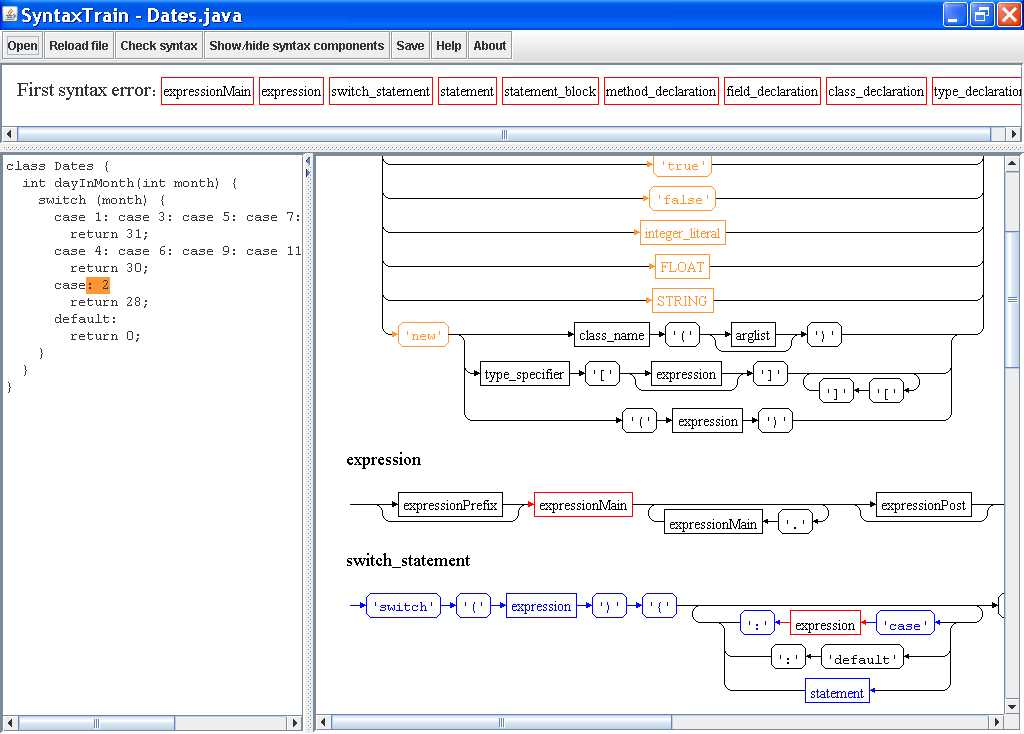
\includegraphics[width=.8\textwidth,keepaspectratio=fixed]{switchCase.png}
\end{center}
\caption{The Date class syntax error displayed by \st{}}\label{fig.scr}
\end{figure}

\begin{figure}[htbp]
\begin{center}
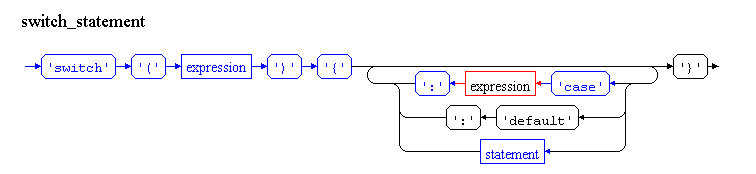
\includegraphics[width=\textwidth,keepaspectratio=fixed]{switchStatementDiagram.png}
\end{center}
\caption{The rule for the \texttt{switch} statement}\label{fig.switch}
\end{figure}

From the left pane we know that there is a problem with the code that
follows the keyword \texttt{case}. The right pane shows that the error occurred when parsing
\texttt{expressionMain} as part of \texttt{Expression}. The yellow
elements in the first diagram show what the parser was expecting, but
there does not seem to be a problem with any expression, so we look down
to the syntax diagram for the \texttt{switch\_statement}, shown
magnified in Figure~\ref{fig.switch}.

Trace through this diagram; every element is blue until we reach the
element after the keyword \texttt{case}. Clearly, the parser was
expecting an expression, but instead we have written the colon before
the expression (the integer literal \texttt{2}) instead of after it.
Modify the source code and revalidate; the error is gone!

\subsection{Example 2}

Look at the code in Figure~\ref{importInsideClassCode} which writes a
string to a file.

\begin{figure}[htbp]
\begin{center}
\begin{lstlisting}[language=Java]
class FileWriterHelper {
  import java.io.*;
 
  public void writeTextToFile( String text, File file ) {
    try {
      BufferedWriter out =
        new BufferedWriter(new FileWriter(file));
      out.write(text);
      out.flush();
    }
    catch (IOException e) {
      System.out.println("Text was not written to file!");
    }
  }
}
\end{lstlisting}
\end{center}
\caption{Example 2}\label{importInsideClassCode}
\end{figure}

Figure~\ref{fileWriterHelperScreenshot} shows a screenshot of the code
opened in \st{}. The left pane shows that the error occurred while
parsing the import statement.

\begin{figure}[htbp]
\begin{center}
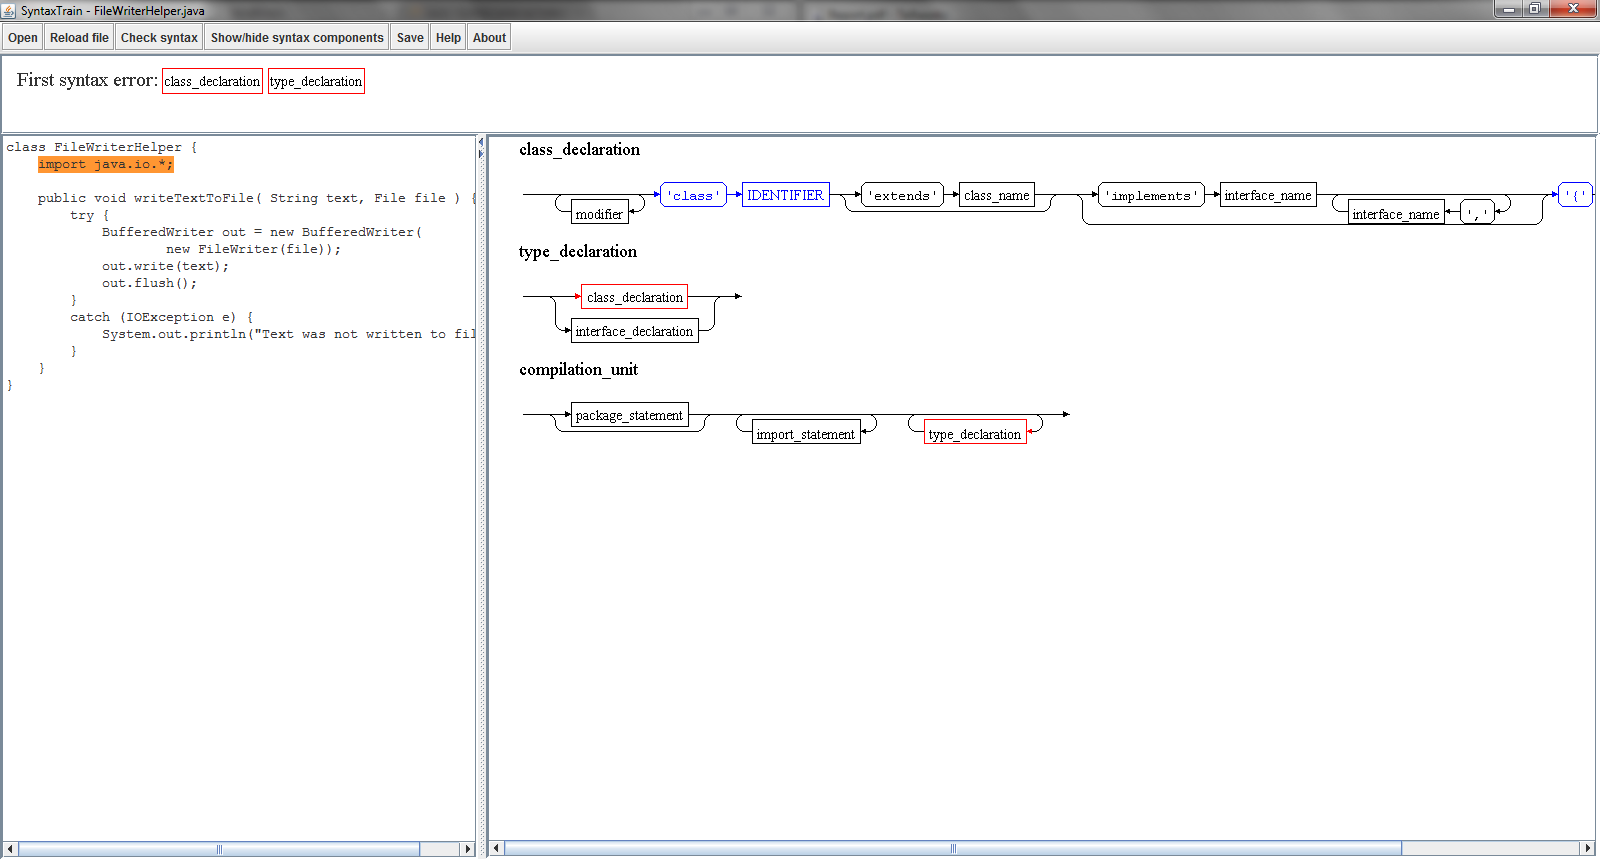
\includegraphics[width=.8\textwidth,keepaspectratio=fixed]{fileWriter.png}
\end{center}
\caption{FileWriterHelper opened in \st{}}\label{fileWriterHelperScreenshot}
\end{figure}

\begin{figure}[htbp]
\begin{center}
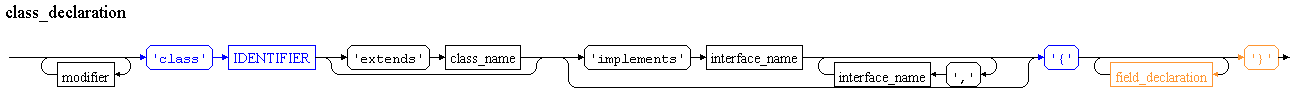
\includegraphics[width=\textwidth,keepaspectratio=fixed]{fileWriterClassDeclaration.png}
\end{center}
\caption{The \texttt{class\_declaration} statement shown by \st{}}\label{fileWriterClassDeclaration}
\end{figure}

In the right pane the top diagram is \texttt{class\_declaration}
(Figure~\ref{fileWriterClassDeclaration}). This diagram shows that only
\verb+}+ and \texttt{field\_declaration} are legal to write at this
point. The former is not relevant since the parsing has not reached the
end of the class.

However, a \texttt{field\_declaration} must be a method, a constructor,
a variable declaration or a static initializer (If you do not remember
this, select \texttt{Show/hide syntax components} (F10) and click the
\texttt{field\_declaration} component). It follows that \texttt{import}
is illegal at this point. Looking down through the diagrams, we see that
\texttt{compilation\_unit} can accept an \texttt{import\_statement}, but
before the \texttt{type\_declaration}, which is an interface or a class.
Moving the import statement before the class declaration solves the
problem.

\subsection{Example 3}

Figure~\ref{calculatorSourceCode} shows a fragment of a calculator
class, including a method for the operation square root. The method
saves the result in the variable \texttt{sum}. This code contains no
syntax errors.

\begin{figure}[htbp]
\begin{center}
\begin{lstlisting}[language=Java, numbers=left,numbersep=-10pt]
  class Calculator {
	int sum;
	
	public void sqrt() {
		int s = 2;
		while ((s)*(s) <= sum) {
			s = s + 1;
		}
		sum = s - 1;
	}
	public Calculator(int initialValue) {
		sum = initialValue;
	}
   }
\end{lstlisting}
\end{center}
\caption{Example 3}\label{calculatorSourceCode}
\end{figure}

Suppose now that you forget the semicolon at the end of line 7.
Figure~\ref{calculatorScreenshotMissingSemicolon} shows a screenshot of
\st{}; it is clear that the semicolon is missing, since expression was
matched correctly and semicolon is now the only legal possibility.

\begin{figure}[htbp]
\begin{center}
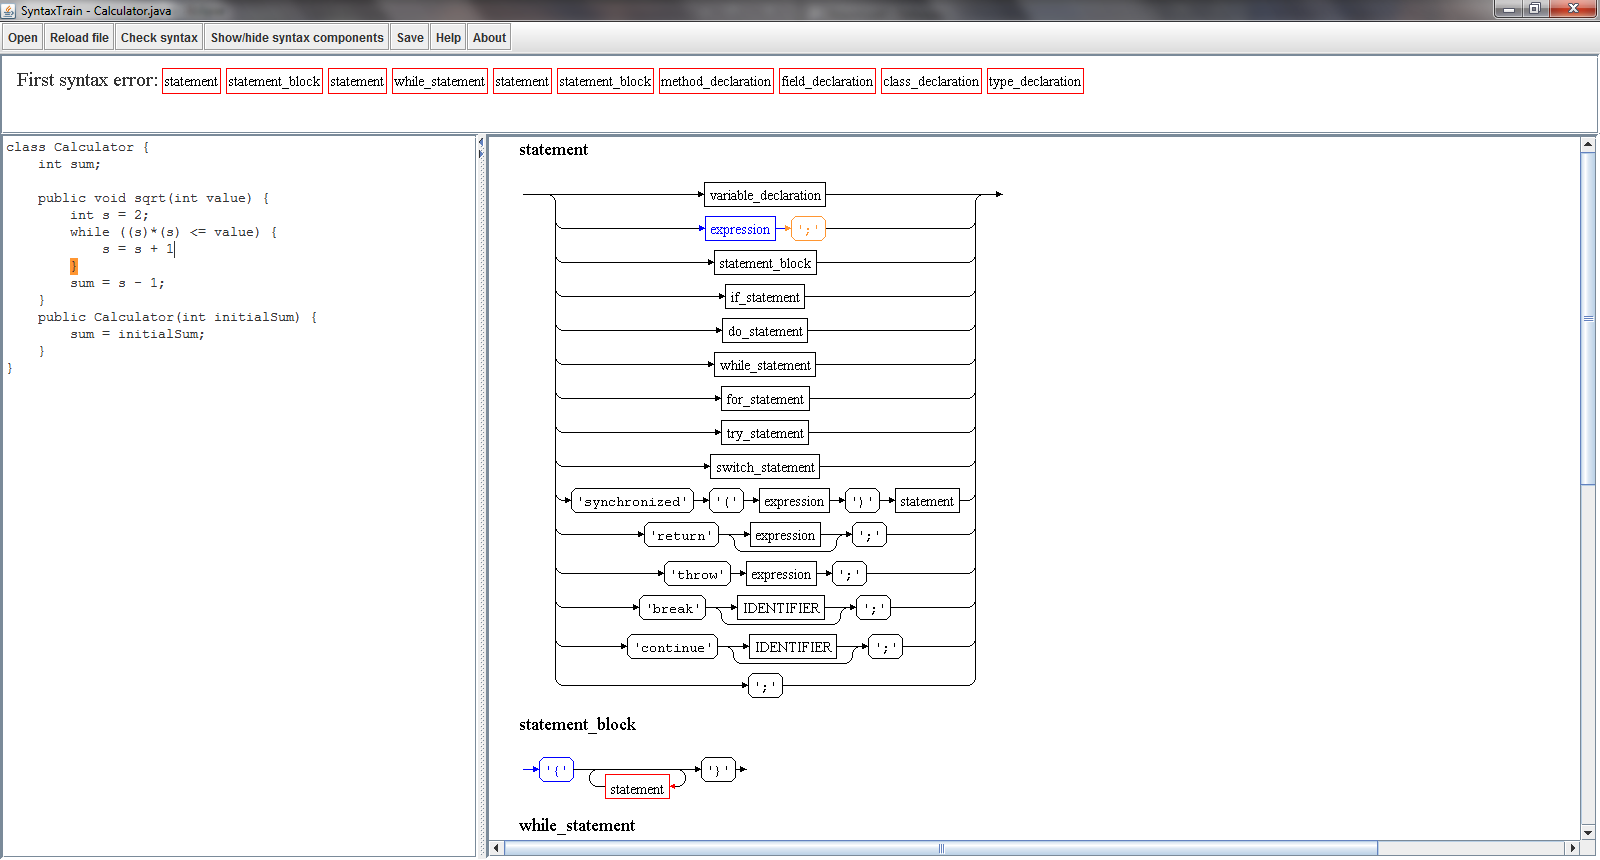
\includegraphics[width=.8\textwidth,keepaspectratio=fixed]{calculatorMissingSemicolon.png}
\end{center}
\caption{Screenshot of a syntax error where a semicolon is missing}\label{calculatorScreenshotMissingSemicolon}
\end{figure}

Suppose, instead, that the user forgets the left brace \textbf{\{} for
the \texttt{while}-statement at line 6.
Figure~\ref{calculatorMissingParenthesis} shows this error displayed in
\st{}. From the highlighted source code in the left pane, it is seen
that the error occurred after the assignment to the variable
\texttt{sum}. The right pane shows that the error occurred while parsing
\texttt{field\_declaration}, which means that the compiler expects a
method, constructor, variable declaration or static initializer at this
point. What the user intended to write at that point is neither of
those, but an expression. Therefore we go on to the next diagram, in
order to find something familiar and then backtrack.

The next diagram is \texttt{class\_declaration}, see
Figure~\ref{calculatorClassDeclaration}. This is where the Calculator
class is defined. Tracing through this diagram we see that the error
occurs while inside the brace and parsing \texttt{field\_declaration},
which we already knew. Since the error occurred at the level of the
\texttt{field\_declaration}, and not inside the method, that means that
for some reason we are \emph{outside} the function. A careful inspection
of the code will show that the brace that should have closed the
\texttt{while}-statement actually closed the function instead.

\begin{figure}[htbp]
\begin{center}
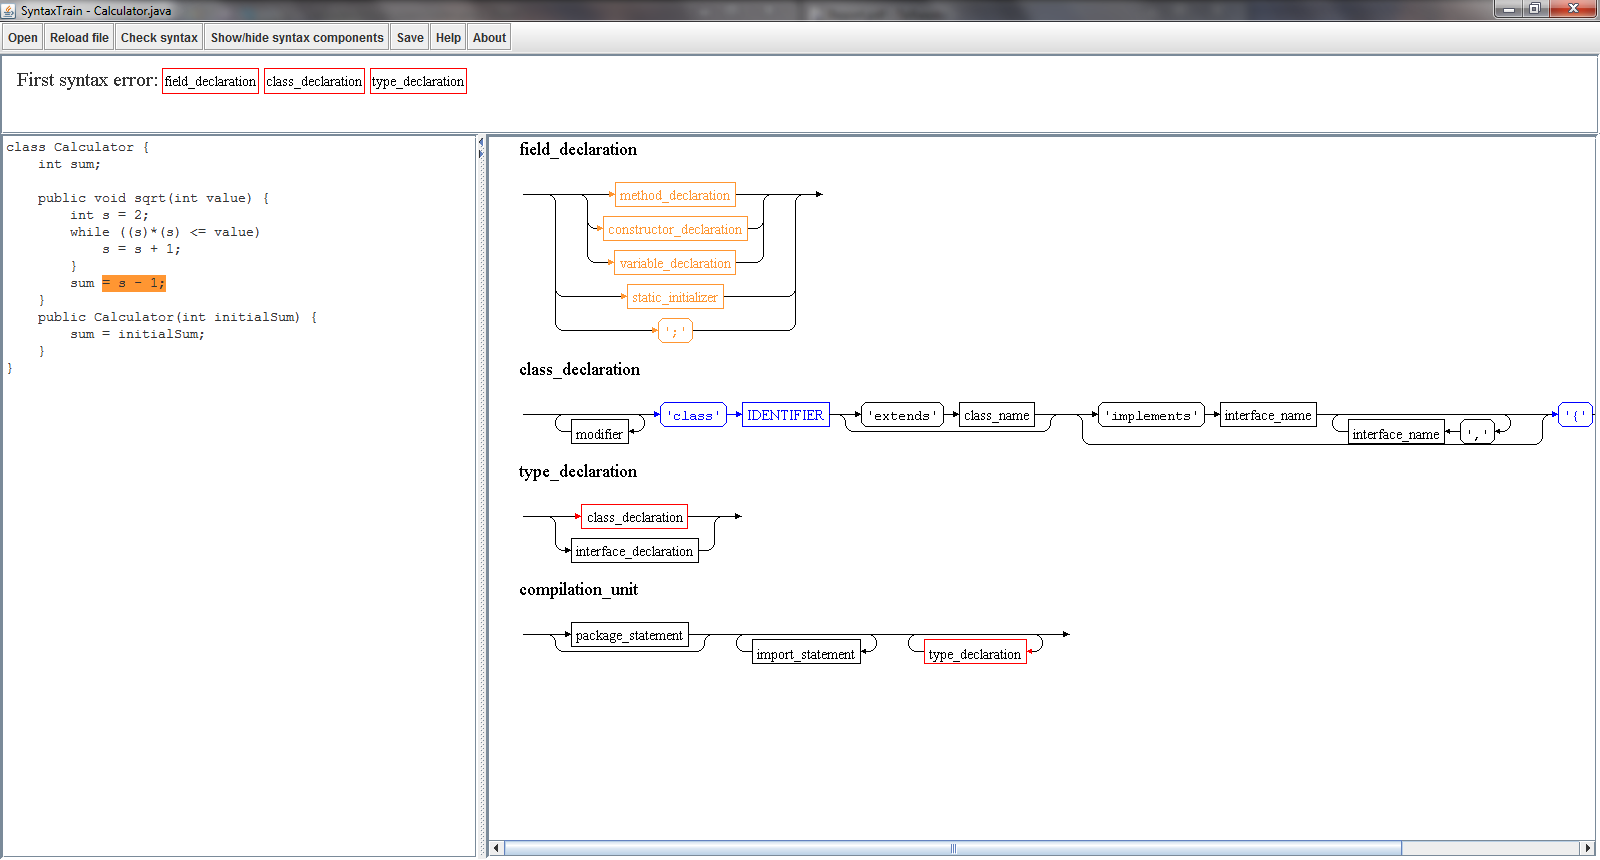
\includegraphics[width=\textwidth,keepaspectratio=fixed]{calculatorMissingParenthesis.png}
\end{center}
\caption{Screenshot of a syntax error where the \textbf{\{} is missing}\label{calculatorMissingParenthesis}
\end{figure}

\begin{figure}[htbp]
\begin{center}
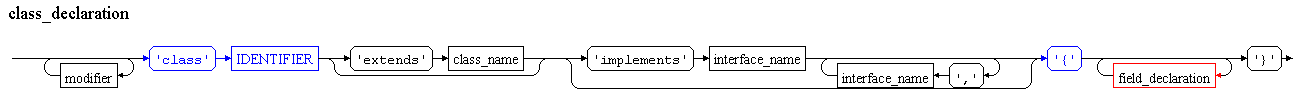
\includegraphics[width=\textwidth,keepaspectratio=fixed]{calculatorClassDeclaration.png}
\end{center}
\caption{The \texttt{class\_declaration} statement shown by \st{}}\label{calculatorClassDeclaration}
\end{figure}

\newpage

\section{Adapting \st{} for a new language}\label{s.bnf}

The BNF compiler is a tool that reads a text file containing the grammar
of a language in BNF and creates a grammar file that can be
used by \st{}. The distribution includes the file
\texttt{javagrammar.bnf} with the BNF for \jv{}.
To create the grammar file for \st{}, run:
\begin{verbatim}
java -jar BnfCompiler.jar bnf-filename
\end{verbatim}
First make sure that the path to your JDK bin directory is specified
in the file \texttt{options.xml}.

There are several limitations that must be followed when preparing a BNF
for use in \st{}:

\begin{itemize}
\item The first rule is the starting rule.
\item The BNF may not be left recursive.
\item The BNF must be decidable, that is, there must be
only one way to match a given string.
\end{itemize}

The following rules have been pre-programmed into the grammar file:
\begin{itemize}
\item IDENTIFIER: any string consisting of letters, underscore and
numbers, and starting with a letter or underscore.
\item INT: integer literals.
\item FLOAT: float literals.
\item HEX: hex literals, which must start with a number as in 0FE.
\item STRING: strings delimited by quotation marks.
\item HEX\_DIGIT: a single-digit hex literal.
\end{itemize}

Additionally the following are automatically ignored:
\begin{itemize}
\item Comments: delimited by /* and */, or // until end of line.
\item Whitespace: new lines, line feed, tabs and spaces.
\end{itemize}

\section{Software documentation}\label{s.doc}

\st{} uses the \an{} parser generator \url{http://www.antlr.org/} in
order to convert a BNF into a stack of rules. This stack of rules are used to
create another \an{} file that is able to verify the language specified
by the BNF and return a stack trace in case there is a syntax error.

\cp{} \url{http://clapham.sourceforge.net/} is used to draw the syntax
diagrams. It has been modified to support specifying colors and fonts,
along with some minor bugfixes.

The \st{} software consists of two major components: the GUI and the
kernel, which communicate through two interfaces: \texttt{GuiApi}
\texttt{KernelApi}. The kernel manages the interaction with \an{} and the modelling part of \cp{}; that is, to describe to \cp{} how the diagrams are structured and which components should be highlighted.

The kernel consists of the following classes:
\begin{itemize}
\item \textbf{GrammarBase}: Reads/writes source code and loads grammar files.
\item \textbf{GrammarCompiler}: Creates syntax nodes used by \cp{}, modelled to match the grammar and colored depending on the stack trace.
\item \textbf{SourceCodeCompiler}: Verifies the source code using \an{} parser and lexer files, loaded by GrammarBase.
\item \textbf{GrammarInterface}: Interface to the kernel, to ensure that calls are made in right order.
\item \textbf{Variables}: Various global variables and constants used by the kernel.
\end{itemize}

The GUI consists of the following classes (graphical components all starts with a lower-case \emph{g}, with the exception of MainScreen):

\begin{itemize}
\item \textbf{Controller}: Handles all gui events, except those of the \texttt{Syntax components} pane.
\item \textbf{Dialogs}: Shows about and help dialogs.
\item \textbf{gErrorTrace}: The top pane that shows a list of rules involved in the error.
\item \textbf{gGrammarDiagram}: Panel containing the diagrams generated by \cp{}, it also calls \cp{} to generate these diagrams.
\item \textbf{gGrammarOptions}: Panel allowing the user to select which diagrams are shown.
\item \textbf{gGrammarPanel}: Panel containing both \texttt{gGrammarDiagram} and \texttt{gGrammarOptions}.
\item \textbf{gSourceCode}: Text pane for showing and highlighting the source code.
\item \textbf{gToolbar}: Toolbar at the top (also registers shortcuts).
\item \textbf{MainScreen}: The main frame.
\item \textbf{Variables}: Various global variables and constants used by the gui.
\end{itemize}

All grammar files contains a parser that extends \texttt{BnfParser}, such that all grammars have a similar interface.

Besides from these classes, a few helper classes are also used. These are \texttt{XmlNode} (reads XML), \texttt{Lock} (concurrent lock, to avoid race-conditions) and \texttt{StdLibrary} (reads files and escapes strings).

The \texttt{BnfCompiler} consists of \texttt{CommandLineTool}, which manages the entire process of generating a grammar file from a BNF.
\texttt{CommandLineTool} uses \texttt{BnfEvaluatorParser} and \texttt{BnfEvaluatorLexer} to read BNF and return a stack of \texttt{Link} to describe the language.
\texttt{BnfEvaluatorParser} and \texttt{BnfEvaluatorLexer} are generated using \an{}, the code can be found in \texttt{BnfEvaluator.g}.
\texttt{Link} is a class, which you can put together with other links, telling that the given link is optional, one of multiple options, a loop running 0+ times, a loop running 1+ times or a simple sequence.

\end{document}
